
\documentclass[a4paper,onecolumn,11pt,unpublished]{quantumarticle}
\pdfoutput=1

%% Bibliography
\usepackage[numbers,sort&compress]{natbib}
\usepackage[nottoc]{tocbibind}

%% Math
\usepackage{amsmath,amssymb,amsthm,bm,amsfonts,mathrsfs}
\usepackage{braket}

%% Figures & tables
\usepackage{graphicx}
\usepackage{booktabs}
\usepackage{tabularx}
\usepackage{siunitx}
\usepackage{float}
\usepackage{subcaption}
\usepackage{caption}
\usepackage{multicol}
\usepackage{multirow}

%% Algorithms & code
\usepackage{algorithm}
\usepackage[noend]{algpseudocode}
\usepackage{minted}     % requires --shell-escape; see README

%% Typography
\usepackage[utf8]{inputenc}
\usepackage[T1]{fontenc}
\usepackage[english]{babel}
\usepackage{hyperref}
\usepackage[babel]{microtype}
\usepackage{csquotes}

%% Layout
\usepackage{wrapfig}
\usepackage{xcolor}
\usepackage{geometry}
\usepackage{fancyhdr}

%% Theorem environments
\newtheorem{theorem}{Theorem}

%% Convenience macros
\newcommand{\QICK}{\textsc{qick}}
\newcommand{\todo}[1]{{\bfseries\color{red}[TODO: #1]}}

%% Abstract style (replaces quantumarticle's abstract to avoid double \maketitle)
\title{}
\renewenvironment{abstract}
    {\small
    \begin{center}
    \bfseries Abstract
    \end{center}
    \quotation}
    {\endquotation}


\begin{document}

\pagenumbering{gobble}
\begin{titlepage}
\vspace*{-1cm}

\begin{center}

\includegraphics[height=1cm]{logos/UB.png}\hspace{1em}

\includegraphics[height=1cm]{logos/Qili.png}\hspace{1em}

\includegraphics[height=1cm]{logos/MQST.png}
\end{center}

\vspace*{2.5cm}
\begin{center}

\large\textsc{MSc Quantum Science and Technology}

\vspace*{1cm}
\large\textsc{Master Thesis}

\vspace*{1cm}

\line(1,0){400}

\vspace*{0.25cm}

\Huge\bfseries\sffamily Toward ML-Based State Discrimination on FPGA in Open-Source Quantum Control Electronics

\vspace*{0.2cm}

\line(1,0){400}

\vspace*{1.5cm}
\large
Author: Ender Jose Barillas Rodriguez

\vspace{0.5cm}
Supervised by: Joel Pérez Díaz

\end{center}

\vfill
\parbox[t]{\linewidth}{%
     NIUB: 23254663         \\
     Faculty of Physics, University of Barcelona      \\
     08028, Barcelona \\
     July 2026
  }

\end{titlepage}

\newpage

\textcolor{white}{p}
\vspace{3cm}
\section*{Acknowledgements}
\pagenumbering{roman}

I would like to thank the team at Qilimanjaro Quantum Tech for their
guidance and support throughout this project.  Special thanks to Joel Pérez Díaz
for supervising this work and to all colleagues who offered
technical help and stimulating discussions.  This thesis was carried out during
an internship at Qilimanjaro from February to July 2026.
\todo{Expand. Thank David A. for reviewing, and Fabio H. and the team for help with the board. Thank classmates. Thank Bruno and the program for letting me take a shot at joining a new field. Thank Arianna for helping me survive in Barcelona. Thank parents as well.}


\newpage

\begin{abstract}
Low-latency and high-fidelity qubit state measurement is essential for
superconducting quantum computing, particularly for enabling mid-circuit
measurements and real-time feedback. Conventional readout techniques rely on
host-side processing, introducing delays that limit measurements to the end of a
quantum circuit. FPGA-based approaches offer a path toward in-situ state
discrimination, but many existing solutions are specialised or tightly coupled to
specific hardware designs.

This thesis presents a general-purpose readout architecture based on the
\QICK{} framework~\cite{Stefanazzi2022}, implemented on a Xilinx ZCU216 RFSoC
platform, that supports both mid-circuit and end-of-circuit quantum state
measurements. The work encompasses full system integration, including FPGA
configuration and remote operation, \QICK{}-based calibration, and the design of
a real-time readout data path. Control and readout waveforms are generated using
Direct Digital Synthesis (DDS), and the role of the analogue front end is
examined to ensure reliable signal transmission and measurement.

Building on this infrastructure, we investigate machine-learning-assisted state
discrimination within \QICK{} to accelerate readout while maintaining accuracy.
Lightweight machine-learning methods suitable for FPGA deployment are evaluated
with respect to latency and computational cost. The resulting architecture enables
low-latency state classification directly on the control hardware, reducing
reliance on host-side processing and providing a unified measurement pipeline for
dynamic quantum circuits.
\end{abstract}

\noindent{\it Keywords}: superconducting qubits, readout, FPGA, QICK, RFSoC,
  dispersive measurement, mid-circuit measurement, machine learning

\newpage

\tableofcontents

\newpage
\pagenumbering{arabic}

\setlength{\headheight}{14pt}
\pagestyle{fancy}
\rhead{Ender Jose Barillas Rodriguez}
\lfoot{MSc Thesis}
\rfoot{Barcelona, July 2026}

%% ----------------------------------------------------------------

%% Chapter 1 — Introduction
\section{Introduction}
\label{sec:introduction}

Quantum computing holds the promise of solving classically intractable problems
in optimisation, simulation, and cryptography.  Among the leading hardware
platforms, superconducting qubits stand out for their relatively fast gate times,
high coherence, and compatibility with existing microwave engineering
infrastructure~\cite{Krantz2019}.  A central challenge that must be overcome on
the road to fault-tolerant operation is \emph{qubit state measurement}: reading
out the quantum information stored in a qubit quickly, accurately, and with
minimal back-action on unmeasured qubits.

\subsection{Motivation}

Classical error correction requires measurements that are not only high-fidelity
but also \emph{fast} relative to qubit coherence times, and — crucially for
quantum error correction — it requires \emph{mid-circuit measurements}: the ability to measure ancilla qubits repeatedly during a quantum algorithm, use the results to extract error syndromes in real time, and continue the computation on the data qubits.  This capability demands a control electronics stack capable of making a state discrimination decision on-chip in microseconds — the timescale of the readout integration window itself — rather than the milliseconds typical of a software round-trip to a host CPU.

Field-Programmable Gate Arrays (FPGAs) offer a compelling solution.  Their
deterministic, sub-microsecond timing enables real-time signal processing close
to the qubit hardware.  Commercial control platforms such as Qblox, Zurich
Instruments, and Quantum Machines already exploit this, providing on-FPGA state
discrimination within closed, proprietary firmware stacks.  However, closed
firmware precludes custom signal processing pipelines: researchers cannot inject
bespoke algorithms — including machine-learning classifiers — into the real-time
decision path.  The Quantum Instrumentation Control Kit
(\QICK)~\cite{Stefanazzi2022} addresses this gap as an open-source FPGA firmware
and software framework that turns Xilinx Radio-Frequency System-on-Chip (RFSoC)
boards into complete qubit controllers, combining fast digital-to-analogue
converters (DACs), analogue-to-digital converters (ADCs), and a tightly
integrated soft-processor into a single compact platform.  Full access to the
programmable logic fabric makes it possible to define the entire readout and
discrimination pipeline, including the integration of custom ML models, in a way
that closed commercial firmware does not permit.

\subsection{Goals and Contributions}

Despite the availability of \QICK{}, assembling a \emph{general-purpose} readout
pipeline from an uncharacterised board to a working single-shot state
discriminator requires integrating many layers: physical wiring, FPGA
configuration, phase calibration, signal optimisation, and machine-learning
post-processing.  The lack of a unified reference implementation makes this
process time-consuming and error-prone, especially for multi-qubit scenarios.

This thesis makes the following contributions:

\begin{enumerate}
      \item \textbf{Full-stack integration} of the \QICK{} framework on a Xilinx
            ZCU216 RFSoC board with an XM655 analogue front-end module, including
            remote operation via a persistent Pyro4 server.

      \item \textbf{Phase-coherent readout calibration}: a systematic procedure for
            measuring and compensating the random DAC–ADC phase offset that arises at
            every board power-on, enabling reproducible IQ measurements across
            sessions.

      \item \textbf{Readout data-path design}: a characterisation of the trade-offs
            between decimated and accumulated readout modes and a complete resonator
            spectroscopy workflow suitable for both single-qubit and multiplexed
            measurements.

      \item \textbf{Real-time feedback primitives}: demonstration of the
            \texttt{condj} conditional-branch primitive on the tProcessor in loopback,
            and design of an active qubit reset sequence combining dispersive readout,
            thresholding, and a calibrated $\pi$ pulse — establishing the
            infrastructure needed for mid-circuit measurement once the board is
            connected to a qubit chip.

      \item \textbf{ML-assisted state discrimination}: offline design and evaluation
            of a lightweight ML discrimination pipeline on existing experimental SSRO
            data, establishing that LDA is near-optimal for integrated IQ inputs, and
            demonstrating via synthetic raw traces that a 1D CNN recovers
            $T_1$-relaxation shots irrecoverable by integration-based methods.  A
            concrete path toward FPGA deployment is outlined.
\end{enumerate}

\subsection{Thesis Outline}

Section~\ref{sec:background} reviews the relevant theory of superconducting
qubits, circuit quantum electrodynamics (cQED), and dispersive readout.
Section~\ref{sec:hardware} describes the hardware platform.
Section~\ref{sec:integration} covers system integration and calibration.
Section~\ref{sec:readout} presents the readout architecture and measurement
workflows.  Section~\ref{sec:feedback} describes real-time feedback and
mid-circuit measurement.  Section~\ref{sec:ml} evaluates machine-learning-based
state discrimination.  Section~\ref{sec:conclusions} summarises the results and
outlines future directions.

%% Chapter 2 — Theoretical Background
\section{Theoretical Background}
\label{sec:background}

\subsection{Superconducting Qubits}

Superconducting qubits are anharmonic LC oscillators whose nonlinearity is
provided by one or more Josephson junctions~\cite{Krantz2019}.  The Josephson
junction acts as a nonlinear inductor with energy $E_J\cos\hat{\varphi}$, where
$\hat{\varphi}$ is the superconducting phase across the junction and $E_J$ is the
Josephson energy.  Combined with a shunt capacitance $C$ (charging energy
$E_C = e^2/2C$), the system forms an artificial atom with a discrete, anharmonic
spectrum that can be addressed at the transition frequency $\omega_{01}$. Several qubit designs have been developed that exploit this anharmonicity in different parameter regimes; this thesis is primarily concerned with two: the transmon and the fluxonium.

\paragraph{Transmon.}
The transmon~\cite{Koch2007} operates deep in the regime $E_J \gg E_C$, making
its energy levels insensitive to charge noise.  Its transition frequency lies
typically in the \SIrange{4}{8}{\giga\hertz} range, and its anharmonicity
$\alpha = \omega_{12} - \omega_{01}$ is of order $-E_C/\hbar$, typically a few
hundred \si{\mega\hertz}.

\paragraph{Fluxonium.}
The fluxonium~\cite{Manucharyan2009} replaces the transmon's large capacitor with a
superinductance $L$ (inductive energy $E_L = (\Phi_0/2\pi)^2/L$, where $\Phi_0$ is
the flux quantum), threading the loop with an external flux $\Phi_z$.  The resulting
double-well potential can be tuned between a plasmon regime (near $\Phi_z = 0$) and
a fluxon regime (near $\Phi_z = \Phi_0/2$).  Fluxonium qubits offer long coherence
times and are of particular interest because their readout landscape is richer than
the transmon's: the dispersive shift $\chi$ varies strongly with flux bias, and near
the half-flux sweet spot the two eigenstates carry opposite persistent currents,
giving rise to a large state-dependent dispersive shift that can be exploited for
high-contrast readout~\cite{Manucharyan2009}.

\subsection{Circuit Quantum Electrodynamics}

In the circuit QED (cQED) architecture~\cite{Blais2004}, a qubit is coupled
dispersively to a microwave resonator.  The resonator acts both as a readout bus
and as a filter that protects the qubit from radiative decay into the measurement
chain.  The full Hamiltonian (setting $\hbar=1$) is
\begin{equation}
  \hat{H} = \hat{H}_\text{qubit}
  + \omega_r \hat{a}^\dagger \hat{a}
  + g\,\hat{n}_q (\hat{a} + \hat{a}^\dagger),
  \label{eq:jaynes_cummings}
\end{equation}
where $\omega_r$ is the resonator frequency, $\hat{a}$ ($\hat{a}^\dagger$) is the
resonator annihilation (creation) operator, $g$ is the qubit--resonator coupling
strength, and $\hat{n}_q$ is the relevant qubit operator (charge for capacitive
coupling).

\subsection{Dispersive Readout}
\label{subsec:dispersive}

When $|g_{ij}| \ll |\omega_{ij} - \omega_r|$ for all relevant qubit transitions
$i \leftrightarrow j$, second-order perturbation theory in $g$ yields a
qubit-state-dependent shift of the resonator frequency~\cite{Blais2021}:
\begin{equation}
  \hat{H}_\text{disp} = \left(\omega_r + \sum_i \chi_i \ket{i}\bra{i}\right)
  \hat{a}^\dagger \hat{a},
  \quad
  \chi_i = \sum_{j \neq i}
  \frac{|g_{ij}|^2}{\omega_{ij} - \omega_r}
  - \frac{|g_{ji}|^2}{\omega_{ji} - \omega_r},
  \label{eq:dispersive_shift}
\end{equation}
where $g_{ij} = \braket{i|g\,\hat{n}_q|j}$ and $\omega_{ij} = \omega_j -
  \omega_i$.  The textbook two-level dispersive shift $\chi = \chi_1 - \chi_0$
follows from truncating to the computational subspace, but for fluxonium-class
qubits the straddling regime (where $|g_{12}| \gg |g_{01}|$) makes this
truncation unsafe; higher levels must be included~\cite{Koch2007}.

In practice, one probes the resonator at its bare frequency $\omega_r$ and
observes a state-dependent phase shift of the transmitted or reflected signal.
For a single-qubit system, the resonator sits at $\omega_r + \chi_0$ when the
qubit is in $\ket{0}$ and at $\omega_r + \chi_1$ when in $\ket{1}$, resulting
in an IQ-plane separation that grows with the dimensionless cavity pull
$2|\chi|/\kappa$, where $\kappa$ is the resonator linewidth~\cite{Blais2004}.

\paragraph{Fluxonium dispersive readout.}
For a fluxonium qubit, the dispersive shift landscape is richer than for the
transmon because the qubit spectrum varies strongly with the external flux $\Phi_z$.
Near the half-flux point $\Phi_z = \Phi_0/2$, the double-well potential becomes
symmetric and the two lowest eigenstates carry opposite persistent currents.
The resulting state-dependent coupling to the resonator produces a dispersive shift
$\chi = \chi_1 - \chi_0$ whose magnitude depends strongly on the flux bias point,
making the readout contrast highly tunable.  This flux dependence is a key
motivation for the fluxonium readout optimisation work being pursued in related
projects within the Qilimanjaro team.

\subsection{Direct Digital Synthesis}
\label{subsec:dds}

Direct Digital Synthesis (DDS) generates analogue waveforms by accumulating a
phase register at a fixed clock rate and mapping the instantaneous phase value to
a digital amplitude via a look-up table.  A DDS numerically controlled oscillator
(NCO) produces a tone at frequency
\begin{equation}
  f_\text{out} = \frac{f_\text{clk} \cdot \Delta\phi}{2^N},
\end{equation}
where $f_\text{clk}$ is the system clock, $\Delta\phi$ is the phase increment per
clock cycle, and $N$ is the bit width of the phase accumulator.  DDS avoids the
spur and image problems associated with analogue IQ mixers because all
imperfections are digital and predictable.  In \QICK{}, the tProcessor drives DDS
engines on both the DAC (transmit) and ADC (receive) sides, enabling phase-locked
signal generation and coherent demodulation~\cite{Stefanazzi2022}.

\subsection{State Discrimination}

Following dispersive readout, the measured IQ quadrature amplitudes $(I, Q)$ form
two clusters in the complex plane — one for $\ket{0}$ and one for $\ket{1}$.
Single-shot state discrimination assigns each measurement to one of these
clusters.  The simplest approach is a linear threshold: a hyperplane in the IQ
plane that minimises the total misclassification probability, which for Gaussian
clusters of equal covariance is the perpendicular bisector of the line connecting
the centroids~\cite{Gambetta2007}.  The single-shot readout fidelity is
\begin{equation}
  \mathcal{F} = 1 - \frac{1}{2}\left(p(1|0) + p(0|1)\right),
\end{equation}
where $p(1|0)$ is the probability of assigning $\ket{1}$ given that the qubit was
prepared in $\ket{0}$, and vice versa.  More sophisticated classifiers — quadratic
discriminant analysis, neural networks — can improve fidelity when the clusters are
non-Gaussian or when multi-level leakage is present.

%% Chapter 3 — Hardware Platform
\section{Hardware Platform}
\label{sec:hardware}

\subsection{Xilinx ZCU216 RFSoC}

The Xilinx Zynq UltraScale+ ZCU216 evaluation board~\cite{ZCU216} is built around an RFSoC
device that integrates, on a single chip, a quad-core ARM Cortex-A53 processor,
an FPGA fabric, and 16 RF-DAC and 16 RF-ADC channels with sampling rates up to
\SI{9.85}{\giga S/s} and \SI{2.5}{\giga S/s}, respectively.  At 14-bit resolution,
the converters can directly synthesise and capture signals in the
\SIrange{0}{6}{\giga\hertz} range without an external frequency up-conversion stage,
provided the analogue signal chain is suitably conditioned.

The ZCU216 was chosen for practical reasons rather than as a bespoke control
instrument.  It is a general-purpose RFSoC evaluation board, commercially available
and of the kind a laboratory can readily obtain, and it is one of the platforms
supported by \QICK{}, the open-source control framework at the centre of this work
(Section~\ref{subsec:qick_stack}).  \QICK{} is also moving from a research tool
toward a commercially supported standard: in 2026 the US Department of Energy and
Fermilab finalised an agreement for the control-electronics vendor Qblox to
commercialise and distribute it~\cite{QbloxQICK2026}.  Other RFSoC boards would
also run \QICK{}; the ZCU216 is the one that was available for this project.

The board runs the PYNQ Linux distribution, which exposes the FPGA fabric and the
converters through Python libraries, making it straightforward to implement and
iterate on firmware/software stacks.  Table~\ref{tab:zcu216} summarises the key
specifications relevant to this thesis.

\begin{table}[ht]
      \centering
      \caption{Selected ZCU216 specifications relevant to qubit readout.}
      \label{tab:zcu216}
      \begin{tabular}{lll}
            \toprule
            Parameter        & Value                 & Note              \\
            \midrule
            DAC channels     & 16                    & Differential GSPS \\
            DAC rate         & up to \SI{9.85}{GS/s} & Per channel       \\
            DAC resolution   & 14 bit                &                   \\
            ADC channels     & 16                    & Differential GSPS \\
            ADC rate         & up to \SI{2.5}{GS/s}  & Per channel       \\
            ADC resolution   & 14 bit                &                   \\
            FPGA fabric      & UltraScale+           & 930k LUT          \\
            Processor        & 4$\times$ Cortex-A53  & \SI{1.5}{GHz}     \\
            Operating system & PYNQ Linux            &                   \\
            \bottomrule
      \end{tabular}
\end{table}

\subsection{QICK Software and Firmware}
\label{subsec:qick_stack}

The Quantum Instrumentation Control Kit (\QICK)~\cite{Stefanazzi2022,QICK_github} is an
open-source framework originally developed at Fermilab that turns an RFSoC board
into a self-contained qubit controller.  It consists of two layers:

\paragraph{Firmware.}
The digital logic loaded onto the FPGA, built from reusable hardware modules
(\emph{IP blocks}) using Vivado, AMD/Xilinx's FPGA design software.  Vivado
compiles a description of the desired logic into a \emph{bitstream}, the
configuration file that programs the FPGA fabric into the required circuit at
power-on.  The \QICK{} firmware comprises:
\begin{itemize}
      \item \textbf{Signal generators}: DDS-based waveform engines that drive the
            DACs with arbitrary envelopes, constant tones, or flat-top pulses.
            Generator 0 (the \texttt{axis\_signal\_gen\_v6} engine, DAC tile 2 block 0)
            is used as the primary readout generator throughout this work.
      \item \textbf{Readout blocks}: ADC-side DDS demodulators that down-convert the
            received signal to baseband.  Each readout block provides both a decimated
            output (time-domain I/Q waveform) and an accumulation buffer (averaged I/Q
            pair).  Readout channel 0 (ADC tile 2 block 0) receives the returning tone.
      \item \textbf{tProcessor V2}: a soft-processor that orchestrates pulse timing
            with nanosecond precision.  It executes a custom instruction set including
            direct memory writes (\texttt{memri}), register arithmetic (\texttt{mathi},
            \texttt{regwi}), conditional branches (\texttt{condj}), and pulse triggers.
            The ZCU216 uses the 64-bit variant of the tProcessor, which extends the
            original 32-bit design with wider arithmetic and richer branching.
\end{itemize}

\paragraph{Software.}
A Python library (the \texttt{qick} package) that runs on the ARM core and
exposes high-level classes for writing and running experiments:
\begin{itemize}
      \item \texttt{QickSoc}: instantiates the full hardware stack, loads the
            bitstream, and provides access to the converters and tProcessor.
      \item \texttt{AveragerProgramV2} (from \texttt{qick.asm\_v2}): the base class
            for measurement sequences on the tProcessor-V2 firmware used here.  A
            program subclasses it and defines \texttt{\_initialize()}, which declares
            the generators and readouts and registers named pulses, and
            \texttt{\_body()}, which plays those pulses, triggers the readout, and
            advances time with \texttt{delay\_auto()}.  Parameter sweeps run either
            inside the FPGA via \texttt{add\_loop()} or across separately compiled
            programs from a Python loop (Section~\ref{subsec:spectroscopy}).
\end{itemize}

In this work the board was accessed over SSH and driven from Jupyter notebooks
running in the on-board PYNQ environment, which is how all the experiments
reported here were carried out.

\subsection{XM655 Analogue Front-End Module}
\label{subsec:xm655}

The ZCU216's RF converters use differential signalling on High-Density (HD)
headers (the DAC and ADC used here sit on JHC3 and JHC7).  The XM655 module is Xilinx's daughter-card
solution: it provides BALUN (balanced-to-unbalanced) transformers that convert the
differential DAC outputs and ADC inputs to/from single-ended SMA ports, along with
optional filtering.

The key constraint introduced by the XM655 in this work is its bandwidth: the
BALUNs cover \SIrange{10}{6000}{\mega\hertz}, so resonator frequencies above
\SI{6}{\giga\hertz} require connections directly on the HD header pins using pigtail
cables.  Those tones also fall in the DAC's second Nyquist zone, so the generator is
run with \texttt{nqz=2} to synthesise them; this, together with the balun rolloff,
is why the highest resonators are reached by bypassing the XM655 baluns.

The loopback path used for calibration experiments consists of:
DAC tile 2 blk 0 (JHC3) $\to$ HD-SMA pigtail $\to$ BALUN $\to$ SMA cable
$\to$ BALUN $\to$ HD-SMA pigtail $\to$ ADC tile 2 blk 0 (JHC7).

Figure~\ref{fig:system_topology} shows the high-level signal flow from the
tProcessor to the qubit chip and back.

\begin{figure}[t]
      \centering
      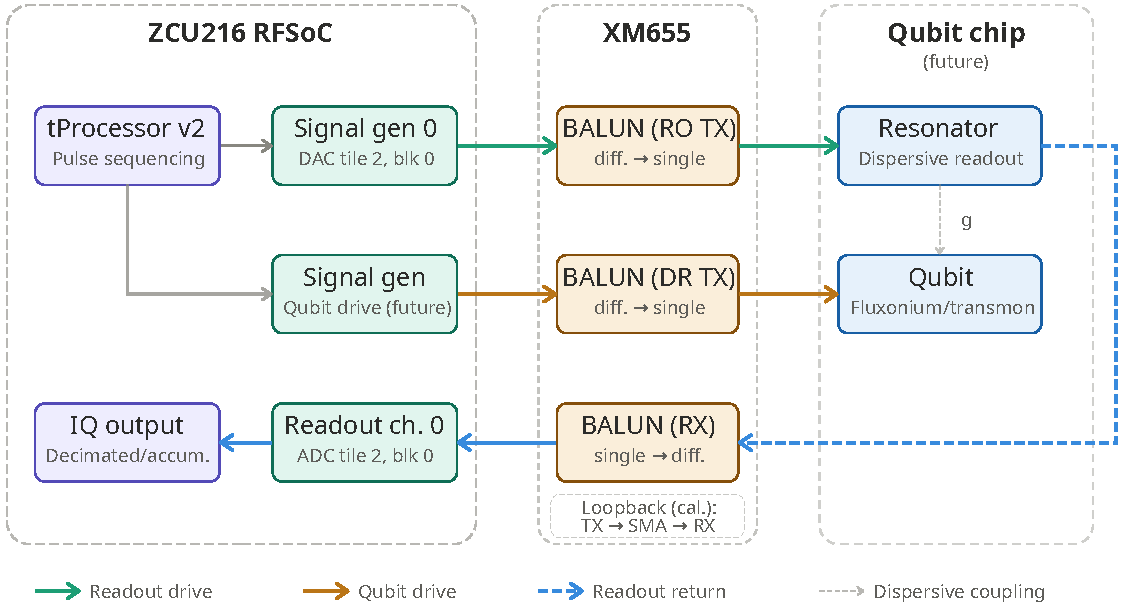
\includegraphics[width=0.92\columnwidth]{figures/system_topology}
      \caption{System signal chain for the \QICK{}-based readout platform.  The
            tProcessor V2 sequences pulses on two generator channels: the readout
            generator drives the readout tone through the XM655 TX BALUN to the
            resonator, and a second generator drives the qubit directly via a second
            TX BALUN channel for $\pi$-pulse control.  The reflected readout tone
            returns through the XM655 RX BALUN to the readout ADC and is demodulated
            to an IQ pair (the channel and port numbers are those of
            Table~\ref{tab:channels}).  The XM655 BALUNs cover
            \SIrange{10}{6000}{\mega\hertz}; resonator frequencies above
            \SI{6}{\giga\hertz} require direct HD-header pigtail connections,
            bypassing the XM655.  The qubit chip and its connections are shown as a
            design target; the board was not connected to a qubit chip within the
            scope of this work.  Calibration experiments use the loopback path
            (TX~BALUN $\to$ SMA cable $\to$ RX~BALUN) shown inside the XM655
            container.}
      \label{fig:system_topology}
\end{figure}

%% Chapter 4 — System Integration
\section{System Integration}
\label{sec:integration}

\subsection{FPGA Configuration and Board Bring-up}

The ZCU216 boots the PYNQ Linux image from an SD card.  After boot, the
\QICK{} bitstream is loaded onto the FPGA fabric by instantiating a
\texttt{QickSoc} object in Python, which calls the PYNQ overlay loader and
configures all IP blocks.  Because the RFSoC converters are controlled through
AXI (Advanced eXtensible Interface) register maps rather than external
chip-select lines, initialisation is
entirely software-driven.

The board is accessed over SSH, and experiments are run from Jupyter notebooks
served from the on-board PYNQ environment.  A single \texttt{QickSoc} instance,
created once per session, loads the bitstream and exposes the converters and
tProcessor to the notebook; the phase calibration of
Section~\ref{subsec:phase_calib} then holds for the remainder of that session.

\subsection{Channel Mapping}

The \QICK{} firmware assigns each physical DAC output to a numbered
\emph{generator channel} and each physical ADC input to a numbered
\emph{readout channel}.  This assignment is specific to the firmware build:
different bitstreams expose different channel counts and even renumber the same
physical port.  The experiments here used the tProcessor v2 firmware build
\texttt{2024-09-03\_216\_tprocv2r21\_demo}~\cite{QICKtprocv2}; Table~\ref{tab:channels}
lists the generator and readout channels used, with their physical ports.

\begin{table}[ht]
\centering
\caption{QICK channel mapping used on the ZCU216 (tProcessor v2 build).}
\label{tab:channels}
\begin{tabular}{llll}
\toprule
\QICK{} Channel & Physical Port & HD Header & Function \\
\midrule
Generator 0 (\texttt{axis\_signal\_gen\_v6}) & DAC tile 2, blk 0 & JHC3 & Readout drive \\
Readout 0                                    & ADC tile 2, blk 0 & JHC7 & IQ acquisition \\
\bottomrule
\end{tabular}
\end{table}

A second path (generator 3, the \texttt{axis\_sg\_mux8\_v1} multiplexed engine, into
readout 6 on JHC8) was also exercised, to compare a filtered against an unfiltered
front end; the single \texttt{axis\_signal\_gen\_v6} path above is the one used for
the measurements reported here.

\subsection{Phase Calibration}
\label{subsec:phase_calib}

Each time the ZCU216 is powered on or the FPGA bitstream is reloaded, the DDS
oscillators in the DAC and ADC blocks boot with a random mutual phase offset
$\phi$.  Without compensation, IQ measurements rotate unpredictably between
sessions, making it impossible to compare results across power cycles.

\paragraph{Phase model.}
A loopback tone from the readout DAC to the readout ADC measures $\phi$ at a given
frequency.  Because the two oscillators are effectively separated by a fixed time
delay $\tau$ (the total group delay around the loopback path), the phase
offset scales linearly with frequency:
\begin{equation}
  \phi(f) = \phi_0 - 360^\circ \cdot \tau \cdot f,
\label{eq:phase_model}
\end{equation}
where $\phi_0$ is a constant offset and $\tau$ is extracted from the fit.
The fitted $\tau$ reflects the combined pipeline delay of the DAC and ADC signal
chains, including the digital up- and down-conversion stages (DUC/DDC) and internal
FIFOs, rather than the physical cable propagation delay, which for a bench loopback
of 1--2\,m contributes only a few nanoseconds.

\paragraph{Calibration procedure.}
The phase calibration sweeps a range of frequencies $f_i$ near the target readout
frequency, records the averaged IQ phasor at each point, and extracts
$\phi_i = \arg\langle I + jQ \rangle$.  The pair $(\phi_0, \tau)$ is then fitted
using \texttt{scipy.optimize.least\_squares}, taking care to handle the
$0^\circ/360^\circ$ phase wrap correctly.  The fit is considered reliable when
the signal-to-noise ratio satisfies $|\text{mag}| \gg \text{RMS}$ (e.g.
$637 \gg 1.8$~ADU in a typical calibration run), where ADU denotes analog-to-digital
units, the raw integer output of the ADC.

The resulting \texttt{res\_phase} value:
\begin{equation}
  \phi_\text{res} = \phi_0 - 360^\circ \cdot \tau \cdot f_\text{res}
\end{equation}
is stored in the experiment configuration dictionary and passed to the readout
pulse via \texttt{soccfg.deg2reg(res\_phase)}, which converts degrees to the
integer register format expected by the tProcessor.  This calibration must be
re-run after every board reboot or bitstream reload, but remains valid throughout
a measurement session.

\paragraph{Measurement cadence.}
A summary of the recommended start-of-session checklist is:
\begin{enumerate}
  \item Power on and wait for PYNQ to boot ($\approx$\SI{60}{\second}).
  \item Connect the loopback (readout DAC $\to$ balun $\to$ SMA $\to$ balun $\to$
        readout ADC) and run the phase calibration notebook.
  \item Identify the correct \texttt{adc\_trig\_offset} using decimated readout,
        then switch to accumulated readout for all data-taking
        (Section~\ref{subsec:decimated_vs_accum}).
  \item At session end, call \texttt{soc.reset\_gens()} to halt all running
        generators.
\end{enumerate}

%% Chapter 5 — Readout Architecture
\section{Readout Architecture}
\label{sec:readout}

\subsection{DDS-Based Signal Generation}

\QICK{} avoids the analogue mixing of a standard heterodyne readout chain, in
which a local oscillator (LO) up-converts a baseband envelope to the resonator
frequency $f_r$ at the price of image products, LO leakage, and IQ imbalance
correction.  Both the readout drive and the
demodulation reference are instead produced by the on-chip DDS engines, which operate at
the direct output frequency of the RFSoC converters (up to several GHz).  The
waveform generated for qubit readout has the form
\begin{equation}
  s(t) = A \cdot \text{env}(t) \cdot \cos(2\pi f_r t + \phi_\text{res}),
\end{equation}
where $\text{env}(t)$ is the pulse envelope (constant, Gaussian, Derivative
Removal by Adiabatic Gate (DRAG), etc.),
$f_r$ is programmed directly into the DDS frequency register, and
$\phi_\text{res}$ is the phase correction from calibration.  The residual
imperfections are digital: quantisation and DDS phase-truncation spurs, which are
deterministic and can be mitigated by appropriate filtering and sample-rate
choice, plus random clock jitter.

\subsection{Decimated vs. Accumulated Readout}
\label{subsec:decimated_vs_accum}

After the ADC samples the incoming signal, the \QICK{} readout block demodulates
it by multiplying with the NCO reference tone and low-pass filtering.  Two output
modes are available:

\paragraph{Decimated readout.}
Stores the full time-domain I/Q waveform over the readout window (e.g.\ 1000
samples).  This is essential for setup: it reveals when the readout pulse arrives
relative to the trigger (\texttt{adc\_trig\_offset}), whether the integration
window is correctly positioned, and whether the signal shape is as expected.  The
per-sample noise on the decimated output is $\sim$\SI{1.9}{ADU} RMS; this is the
raw sample-level noise floor, distinct from the per-shot integrated IQ noise
reported for accumulated readout below.

\paragraph{Accumulated readout.}
The FPGA sums all ADC samples within the readout window into a single $(I, Q)$
pair in hardware, one pair per shot.  This is the standard mode for SSRO: each
shot yields one IQ point, and the discrimination classifier operates on that
point.  The per-shot integrated IQ noise is determined by the within-window
averaging over $T_\text{win}$ samples, not by the number of repeated shots.
From the real SSRO data, the per-shot cluster widths are approximately
\SI{0.65}{}--\SI{0.97}{ADU} per quadrature (state-dependent), with an IQ
separation of \SI{2.53}{ADU} and a projected SNR of 2.46, numerically the
Mahalanobis distance between the clusters
(Section~\ref{subsec:integrated_iq}).  The single-shot
assignment fidelity extracted from these clusters is 0.906 (the LDA baseline of
Section~\ref{subsec:integrated_iq}), a typical value for dispersive readout
without a quantum-limited parametric amplifier in the chain.

For applications that do \emph{not} require single-shot resolution, such as
resonator spectroscopy or Rabi calibration, the same shot can be repeated
$N_\text{reps}$ times and the results averaged, reducing the noise on the
\emph{mean} phasor as $1/\sqrt{N_\text{reps}}$:
\begin{equation}
  \sigma_\text{mean} = \frac{\sigma_\text{single}}{\sqrt{N_\text{reps}}}.
\end{equation}
It cannot
be applied to SSRO, since averaging destroys the per-shot state information.

The practical workflow is to find the correct \texttt{adc\_trig\_offset} and
verify signal quality with \texttt{acquire\_decimated()}, then take all data with
\texttt{acquire()} (accumulated): single shots for SSRO, repeat-averaged shots for
spectroscopy and calibration.

\subsection{Resonator Spectroscopy}
\label{subsec:spectroscopy}

The resonator bare frequency $\omega_r$ and linewidth $\kappa$ are found by
sweeping the probe frequency around the estimated resonator frequency and measuring
the transmitted or reflected IQ amplitude.  In \QICK{}, there are two sweep
strategies:

\paragraph{FPGA-internal sweep (\texttt{add\_loop}).}
On the tProcessor v2 firmware a parameter such as the drive frequency can be swept
inside the FPGA with \texttt{add\_loop}, stepping through all points with no Python
round-trips.  However, the readout down-conversion frequency must track the drive to
keep the demodulated signal at baseband, and \texttt{add\_loop} cannot step it: it is
fixed per program.  For spectroscopy, where the two must move together, this sweep
alone is insufficient.

\paragraph{Python outer loop.}
A Python loop instead compiles and runs one \texttt{AveragerProgramV2} per frequency
point, setting the generator and matching readout down-conversion frequencies
together each time (\texttt{add\_readoutconfig} with \texttt{gen\_ch} lets \QICK{}
compute the ADC alias automatically).  The per-point overhead is a few milliseconds,
but it can sweep any parameter, including the readout frequency, and is the approach
used here.  At each point the magnitude $|I + jQ|$ of the accumulated phasor is
recorded; the resonator shows up as the dip (reflection) or peak (transmission) in
the swept response.  The workflow was implemented and validated in loopback, where
the swept response traces the front-end passband; with no device connected, no
resonator dip was measured.

\subsection{Multiplexed Readout}
\label{subsec:multiplex}

For multi-qubit systems, simultaneous readout of several qubits on the same
physical line requires \emph{multiplexed readout}: a broadband probe signal
containing multiple tones at the individual resonator frequencies $\{f_{r,k}\}$~\cite{Heinsoo2018,Walter2017}.
The \QICK{} framework supports this through a \emph{Polyphase Filter Bank} (PFB)
readout mode.

A PFB is a bank of digital bandpass filters implemented as a single, efficient DSP
operation (polyphase decomposition of a prototype filter followed by an FFT).  It
takes the broadband ADC stream and simultaneously demodulates $N$ equally-spaced
frequency channels, analogous to a digital spectrum analyser.  Advantages over
the single-tone DDS approach include:
\begin{itemize}
  \item No need to retune the ADC NCO between qubits.
  \item The per-sample cost of demodulating all $N$ channels scales as $O(\log N)$
        through the shared FFT, rather than the $O(N)$ of $N$ independent
        demodulators.
  \item Sidesteps the ADC-frequency-sweep limitation: each PFB output channel is
        a fixed digital filter, not a tunable DDS.
\end{itemize}

Multiplexed readout via the \QICK{} PFB firmware was not implemented here.  The
single-tone DDS architecture described in
Sections~\ref{subsec:decimated_vs_accum} and~\ref{subsec:spectroscopy} was used
throughout.  A natural next step is to extend the architecture to cover the four
resonator frequencies of one of Qilimanjaro's chips: 6.505, 6.730, 6.978,
and \SI{7.389}{\giga\hertz}.  These frequencies lie above the \SI{6}{\giga\hertz}
upper edge of the XM655 balun passband, so simultaneous multiplexed readout at all
four tones would require direct HD-header connections with discrete baluns and
operation of the RF-ADC above its specified input bandwidth, as
discussed in Section~\ref{subsec:xm655}.  The PFB channel spacing and prototype
filter bandwidth would also need to be verified against the \SI{225}{\mega\hertz}
minimum separation between adjacent resonators in this device.

%% Chapter 6 — Real-Time Feedback and Mid-Circuit Measurement
\section{Real-Time Feedback and Mid-Circuit Measurement}
\label{sec:feedback}

A key motivation for FPGA-based control is the ability to execute
\emph{real-time} conditional logic: perform a measurement, make a decision, and
apply a corrective pulse, all on the FPGA.
This section describes the tProcessor instruction set, demonstrates the
conditional branching primitive, and outlines the active qubit reset protocol.

\subsection{tProcessor Architecture}
\label{subsec:tproc_arch}

The tProcessor is a soft-processor synthesised in the FPGA fabric, with a
custom instruction set tailored to pulse generation and readout sequencing.  In
the original (v1) design~\cite{Stefanazzi2022}, on whose demo firmware the
branching demonstration below was run, each
channel page holds 32 general-purpose 64-bit registers, with cross-page registers
for inter-channel synchronisation.  Dedicated instructions fire the DAC generators
or arm the ADC acquisition windows, while timing instructions advance the schedule:
\texttt{synci} moves the tProcessor clock without touching the channel timelines,
\texttt{sync\_all} aligns all channels, and \texttt{wait\_all} stalls until the
readout windows close.  The primitive that matters for feedback, common to v1 and
the tProcessor v2 build used for the readout experiments
(\texttt{qick\_processor} rev 21: \SI{200}{\mega\hertz} core execution clock,
pulse timing resolved on a \SI{614.4}{\mega\hertz} timing clock), is the conditional
branch \texttt{condj page, reg\_a, op, reg\_b, label}, which jumps to \texttt{label}
when \texttt{reg\_a op reg\_b} holds.

All branching targets are resolved at \emph{compile time} by the Python
assembler: \texttt{label()} records instruction positions as named addresses and
jump targets are backpatched before the program is loaded, so at run time only
integer addresses exist.

\subsection{Conditional Logic Demonstration}
\label{subsec:cond_logic}

The \QICK{} Demo 3 notebook demonstrates the core conditional-branch primitive:
\begin{minted}[fontsize=\small,linenos]{python}
def body(self):
    cfg = self.cfg
    self.trigger(adcs=[cfg["ro_ch"]],
                 adc_trig_offset=cfg["adc_trig_offset"])
    # condj: jump to SKIP_PULSE if number < threshold
    self.condj(0, 2, '<', 1, 'SKIP_PULSE')
    self.pulse(ch=cfg["res_ch"])          # skipped if condition true
    self.label('SKIP_PULSE')
    self.wait_all()
    self.sync_all(self.us2cycles(cfg["relax_delay"]))
\end{minted}

The demo uses the v1-style programming interface (\texttt{body}, \texttt{synci};
Section~\ref{subsec:tproc_arch}), not the tProcessor v2 API used elsewhere
(Section~\ref{subsec:qick_stack}).  Registers 1 and 2 are pre-loaded with the threshold and the test value via
\texttt{regwi}.  When \texttt{number=100, threshold=50}: the condition
\texttt{100 < 50} is false, the pulse fires, and the ADC captures a loopback
signal.  When \texttt{number=10, threshold=50}: the condition is true, the pulse
is skipped, and the ADC trace is flat noise.

\paragraph{Timing subtlety.}
Inside a \texttt{body()} with an open ADC acquisition window, time must be
advanced with \texttt{synci}, not \texttt{sync\_all}: \texttt{sync\_all} advances
all channel timelines to the furthest point, the end of the ADC window, so
subsequent pulses would land after it closes; \texttt{synci} advances only the
tProcessor's internal counter.

\subsection{\texorpdfstring{$\pi$}{π} Pulse Calibration}
\label{subsec:pi_pulse}

A $\pi$ pulse rotates the qubit state by 180° on the Bloch sphere:
$\ket{0} \to \ket{1}$ and $\ket{1} \to \ket{0}$.  It is a fundamental primitive
for qubit initialisation (active reset) and single-qubit gates.  Calibrating it
requires a connected qubit chip; this section describes the procedure that would
be followed once the ZCU216 is connected to a device.

The $\pi$ pulse amplitude is found via a \emph{Rabi experiment}: the qubit drive
pulse amplitude is swept from zero, and the readout signal oscillates between the
$\ket{0}$ and $\ket{1}$ IQ clusters as the qubit is driven through successive
half-turns on the Bloch sphere.  The first amplitude at which the signal fully
crosses to the $\ket{1}$ cluster is the $\pi$ amplitude.  The Rabi sequence is:
\begin{enumerate}
  \item Prepare qubit in $\ket{0}$ (wait $\gg T_1$).
  \item Apply qubit drive pulse at frequency $\omega_{01}$ with variable amplitude
        $A$ and fixed duration.
  \item Read out via the resonator.
\end{enumerate}

The qubit drive tone is at $\omega_{01}$, distinct from the resonator frequency
$\omega_r$ used for readout.  For transmons $\omega_{01}$ is typically
\SIrange{4}{8}{\giga\hertz}; for fluxonium biased near half flux it is far lower,
of order \SIrange{0.1}{1}{\giga\hertz}, which changes the drive-line requirements
but not the sequence described here.  Two separate generator channels
are therefore required: one for readout, one for qubit control.  The
\QICK{} firmware supports this natively: the tProcessor can address both channels
independently with nanosecond timing precision.

\subsection{Active Qubit Reset}
\label{subsec:active_reset}

Active reset rapidly returns the qubit to $\ket{0}$ by measuring its state and
applying a corrective $\pi$ pulse only if the qubit is found in $\ket{1}$~\cite{Reed2010}.  The
\QICK{} tProcessor v2 has all the primitives required to implement this entirely
on-FPGA: the conditional branch demonstrated in Section~\ref{subsec:cond_logic}
provides the decision logic, and the two-channel architecture supports
simultaneous readout and drive.  The following protocol, assembled from these
primitives, would be deployed once the board is connected to a qubit chip:
\begin{enumerate}
  \item \textbf{Dispersive readout}: fire the readout tone and acquire the
        accumulated IQ result.
  \item \textbf{Thresholding}: the readout firmware compares the IQ result against
        a pre-calibrated threshold and writes the binary decision into a
        tProcessor register.
  \item \textbf{Conditional $\pi$ pulse}: \texttt{condj} checks the decision
        register and applies a calibrated $\pi$ pulse on the qubit drive channel
        only if the qubit is in $\ket{1}$.
  \item \textbf{Wait}: allow any residual photons in the resonator to decay before
        starting the experiment.
\end{enumerate}

Because the entire decision-to-pulse path would run inside the tProcessor, the
latency between completing the readout window and firing the corrective pulse is
determined solely by FPGA clock cycles.  For the tProcessor v2 build used here,
with its \SI{200}{\mega\hertz} core execution clock, this latency is of order tens
of nanoseconds.

\subsection{Latency Budget}

Table~\ref{tab:latency} gives an estimated latency breakdown for the active reset
sequence.

\begin{table}[ht]
\centering
\caption{Estimated latency contributions in the active reset loop.}
\label{tab:latency}
\begin{tabular}{lrl}
\toprule
Stage & Latency & Notes \\
\midrule
Readout pulse duration     & \SIrange{0.5}{2}{\micro\second}   & Depends on $\kappa$ \\
ADC integration window     & \SIrange{0.5}{2}{\micro\second}   & \\
FPGA decision (threshold)  & $\sim$\SI{10}{\nano\second}        & A few core cycles \\
Conditional branch         & $\sim$\SI{5}{\nano\second}         & 1 core cycle (\SI{200}{MHz}) \\
$\pi$ pulse duration       & \SIrange{50}{500}{\nano\second}    & Set by drive strength; $\ll T_1$ \\
\midrule
Total (excl. readout)      & $<$\SI{1}{\micro\second}           & \\
\bottomrule
\end{tabular}
\end{table}

The dominant latency is the readout integration window; the digital decision and
conditional fire together contribute less than \SI{100}{\nano\second}, well within
qubit coherence times of \SIrange{10}{100}{\micro\second} for state-of-the-art
fluxonium devices.

%% Chapter 7 — ML-Assisted State Discrimination
\section{ML-Assisted State Discrimination}
\label{sec:ml}

\subsection{IQ Data and the Discrimination Problem}

Each single-shot readout produces an averaged $(I, Q)$ pair, a point in the
complex plane.  Repeating the preparation and measurement builds up two clouds of
such points, one for $\ket{0}$ and one for $\ket{1}$, whose centroids and spreads
depend on the readout power, resonator parameters, and integration time.  As set
out in Section~\ref{subsec:state_discrim}, for ideal Gaussian clusters of equal
covariance the optimal linear boundary is the LDA hyperplane of
Eq.~\ref{eq:lda_boundary}, the perpendicular bisector of the centroid line after
whitening by the common covariance; QDA relaxes the equal-covariance assumption and gives
a curved boundary.  In practice, state-preparation errors, $T_1$ decay during the
readout pulse, and higher-level leakage ($\ket{2}$, $\ket{3}$) distort the clusters
from ideal Gaussians and motivate more expressive classifiers.  Throughout, we
quote the assignment fidelity of Eq.~\ref{eq:fidelity}, equivalently the average
of the two per-class accuracies.

\subsection{Lightweight Classifiers for FPGA Deployment}
\label{subsec:classifiers}

For eventual on-FPGA deployment, the classifier must be computable using only
fixed-point arithmetic and a small number of multiply-accumulate operations.  Three
constraints matter: latency (the decision must complete in a time negligible next
to the readout window and $T_1$, in practice a few hundred nanoseconds at most, so
as not to extend the readout dead time),
resource usage (it must fit in the available DSP slices and block RAM without
displacing the readout and tProcessor logic), and trainability (it must train on a
laptop from a few thousand calibration shots).

With these constraints in mind, three classifier families are considered.  A
\textbf{linear threshold} (LDA) reduces to a single dot product and a
comparison, the minimum possible arithmetic, directly implementable in the
tProcessor's \texttt{mathi} instruction.  A \textbf{quadratic threshold} (QDA)
evaluates a $2\times2$ matrix product (4 multiply-accumulates) and handles
asymmetric cluster covariances.  A \textbf{small MLP} with inputs $(I, Q)$, one
to three hidden layers of 4–64 neurons with ReLU activations, and a sigmoid output
can be computed as a matrix-vector product and fits in $\lesssim 200$ DSP
slices on the ZCU216.  The following sections report results from evaluating
these classifiers offline on existing experimental data; FPGA deployment is
discussed in Section~\ref{subsec:deployment_path}.  For prior work on
neural-network-based discrimination, including multiplexed multi-qubit readout,
see Lienhard et al.~\cite{Lienhard2022}.

\subsection{Experimental Data}
\label{subsec:ssro_data}

The dataset used throughout this chapter is \texttt{SSRO.h5}, collected on a
superconducting qubit device at Qilimanjaro, and retrieved from a database containing data from past experiments.  It contains 2000 single-shot IQ
measurements per prepared state ($\ket{0}$ and $\ket{1}$).  Each shot is a
single $(I, Q)$ pair, the time-averaged quadrature amplitudes over the readout
window.  The acquisition metadata (qubit type, resonator frequency and linewidth,
readout power, integration window, measured $T_1$) was not stored with the IQ
data; this limits how precisely the synthetic traces of Part~III can be
calibrated, and motivates collecting fully documented raw datasets on the ZCU216.
The class statistics
extracted from this dataset are summarised in Table~\ref{tab:iq_stats}.

\begin{table}[ht]
\centering
\caption{IQ blob statistics extracted from \texttt{SSRO.h5}.}
\label{tab:iq_stats}
\begin{tabular}{lrr}
\toprule
Quantity & $\ket{0}$ & $\ket{1}$ \\
\midrule
Centroid $\mu_I$ (ADU)   & $-0.32$ & $-2.10$ \\
Centroid $\mu_Q$ (ADU)   & $+4.50$ & $+6.31$ \\
Width $\sigma_I$ (ADU)    & $0.649$ & $0.874$ \\
Width $\sigma_Q$ (ADU)    & $0.764$ & $0.967$ \\
IQ separation (ADU)       & \multicolumn{2}{c}{$2.53$} \\
IQ correlation            & $-0.587$ & $-0.664$ \\
\bottomrule
\end{tabular}
\end{table}

The negative IQ correlation in both states indicates a rotated noise ellipse,
consistent with a readout tone that is not perfectly aligned to the I axis.  The
data were split 80/20 into training and test sets (3200 / 800 shots) using
stratified sampling.

\begin{figure}[ht]
  \centering
  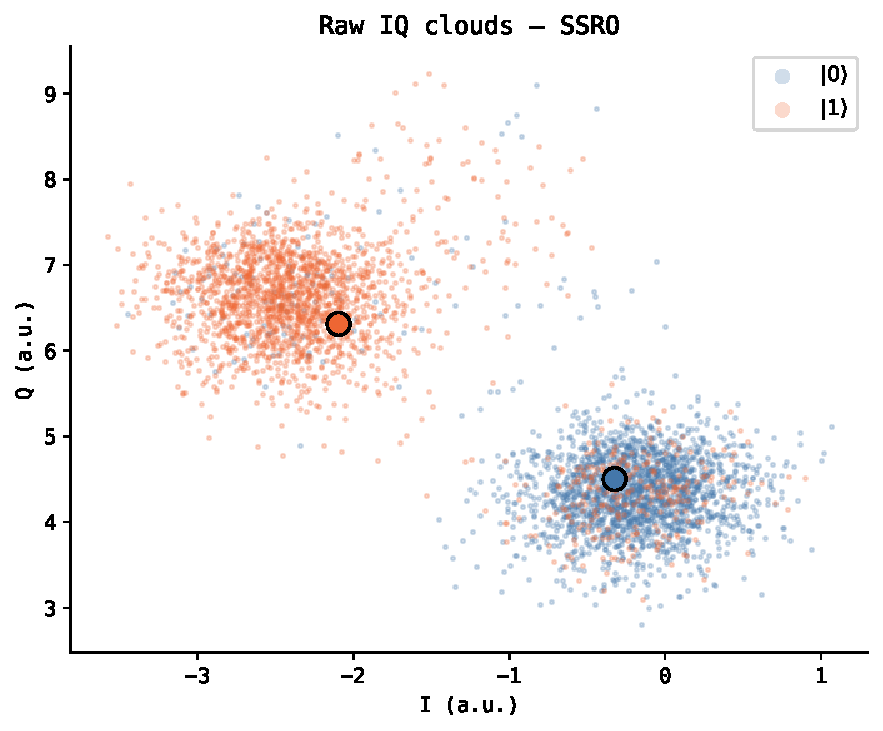
\includegraphics[width=0.55\columnwidth]{code/figures/fig1_iq_scatter}
  \caption{IQ scatter plot of the \texttt{SSRO.h5} dataset (2000 shots per
    state).  Blue: $\ket{0}$; orange: $\ket{1}$.
    Filled circles mark the cluster centroids.  The two clouds are
    well-separated and approximately Gaussian, with the $\ket{1}$ ellipse
    visibly wider, consistent with the $\approx\!1.7\times$ covariance
    asymmetry in Table~\ref{tab:iq_stats}.  The diagonal orientation of both
    ellipses reflects the residual IQ rotation noted in the text.}
  \label{fig:iq_scatter}
\end{figure}

\subsection{Part I: Integrated IQ Discrimination}
\label{subsec:integrated_iq}

LDA, QDA, and a representative MLP (hidden layers 32$\to$16, ReLU) were trained
on the integrated IQ data.  Table~\ref{tab:integrated_results} reports the
assignment fidelity on the held-out test set.

\begin{table}[ht]
\centering
\caption{Assignment fidelity on integrated IQ data (test set, 800 shots).}
\label{tab:integrated_results}
\begin{tabular}{lrrr}
\toprule
Classifier & $\mathcal{F}$ & $\ket{0}$ acc. & $\ket{1}$ acc. \\
\midrule
LDA             & 0.906 & 0.940 & 0.873 \\
QDA             & 0.906 & 0.940 & 0.873 \\
MLP (32$\to$16) & 0.906 & 0.940 & 0.873 \\
\bottomrule
\end{tabular}
\end{table}

All three classifiers achieve identical fidelity, and in fact identical per-class
accuracies: they assign all 800 test shots the same way, because the three decision
boundaries differ
only in regions of the IQ plane that contain no test shots.  The QDA result is the
informative one: the two IQ clouds do \emph{not} share
the same covariance (the
$\ket{1}$ covariance is roughly $1.7\times$ larger than the $\ket{0}$ covariance,
Table~\ref{tab:iq_stats}), so QDA's curved boundary is in principle more expressive
than LDA's linear one.  That it recovers no additional fidelity is explained by the
large cluster separation: the Mahalanobis distance between the centroids is
approximately 2.4, which places the clusters well into the regime where the optimal
boundary is nearly linear regardless of covariance asymmetry.  LDA, QDA, and the MLP
are all saturating the classification capacity of the two-dimensional integrated IQ
input.

The $\ket{0}$ accuracy (94.0\%) exceeds the $\ket{1}$ accuracy (87.3\%),
pointing at a systematic source of $\ket{1}$ misclassification.  This asymmetry
is the first diagnostic signature of $T_1$ relaxation during the readout window,
which causes some $\ket{1}$ shots to produce an integrated IQ that falls in the
$\ket{0}$ blob.

\subsection{Part II: Architecture Search}
\label{subsec:arch_search}

To test whether the LDA–MLP parity in Part I is specific to the (32$\to$16)
architecture, a systematic grid search was performed over 20 MLP configurations
spanning 1–3 hidden layers and 4–64 neurons per layer (17 to 6465 parameters),
evaluated by 5-fold stratified cross-validation.  The LDA baseline quoted here,
$0.898 \pm 0.013$, is the 5-fold CV mean and therefore differs slightly from the
held-out-test value of 0.906 in Table~\ref{tab:integrated_results}.

\begin{table}[ht]
\centering
\caption{Representative architecture grid search results (5-fold CV fidelity);
         see Figure~\ref{fig:grid_search} (Appendix~\ref{appendix:ml}) for all 20
         configurations. LDA baseline:
         $0.898 \pm 0.013$.  No MLP architecture exceeds LDA.}
\label{tab:arch_search}
\begin{tabular}{lrrc}
\toprule
Architecture & $\mathcal{F}$ (CV) & $\pm$ std & $\Delta$ vs.\ LDA \\
\midrule
(4,)         & 0.897 & 0.012 & $-0.001$ \\
(64,)        & 0.897 & 0.012 & $-0.001$ \\
(8, 8)       & 0.896 & 0.012 & $-0.002$ \\
(32, 16)     & 0.897 & 0.012 & $-0.001$ \\
(64, 64)     & 0.897 & 0.012 & $-0.001$ \\
(64, 64, 32) & 0.897 & 0.012 & $-0.002$ \\
\bottomrule
\end{tabular}
\end{table}

The fidelity landscape is flat: no architecture, across three orders of magnitude
in parameter count, improves on LDA.  This is not a failure of the models but a
statement about the data, and it follows directly from Part~I: LDA already finds a
near-Bayes-optimal boundary, and no classifier can improve on it from the same
two-dimensional integrated IQ features.

Further improvement must therefore come from richer inputs, not a more expressive
classifier.  The $\ket{1}$ accuracy deficit diagnosed in Part~I points to the
mechanism: $T_1$ relaxation mid-shot.

\subsection{Part III: Raw-Trace CNN}
\label{subsec:cnn}

\subsubsection{Motivation and the T1 Relaxation Problem}

As established in Section~\ref{subsec:ml_background}, no classifier operating on
integrated IQ can recover a shot in which $T_1$ relaxation occurs mid-window: the
integrator averages over both signal levels and the point lands between the two
clusters, destroying the information about the prepared state.  The raw ADC trace,
by contrast, encodes the relaxation time $t^*$ directly as a step in the IQ
trajectory, and a 1D CNN can detect this step and recover the correct label.
Convolutional filters are suited to exactly this kind of local temporal structure,
which pointwise classifiers cannot exploit.

Demonstrating this directly would require a real dataset of raw ADC traces from a
qubit device, and no such dataset was available for this thesis.  The qubit
processor was not accessible in time, so Parts~I and~II used existing single-shot
IQ data from Qilimanjaro's databases (Section~\ref{subsec:ssro_data}).  That data
is \emph{integrated} IQ, one $(I,Q)$ pair per shot: the per-sample time traces are
discarded on the FPGA, since integrated IQ is the standard readout product, so no
raw traces existed to train on.  Acquiring raw traces
is precisely one of the reasons for setting up the ZCU216 (its
\texttt{acquire\_decimated} mode returns the full time trace); collecting them is
part of the future work this thesis prepares for.

In the meantime, Part~III works with \emph{synthetic} traces.  Here ``synthetic''
does not mean invented: each trace is built from the real device's measured IQ
statistics (the centroids and noise covariances of Table~\ref{tab:iq_stats}) and
shaped into the time-resolved signal a raw acquisition would produce, including the
mid-shot relaxation step.  This lets the full discrimination pipeline, from raw
trace to trained CNN, be developed and validated now, so that it is ready to run on
real traces as soon as a chip is available.

\subsubsection{Synthetic Trace Model}

Each shot is modelled as a noisy cavity response, following the standard
dispersive-readout signal model in which the intracavity field rings up toward its
steady-state value at a rate set by the resonator linewidth
$\kappa$~\cite{Blais2021,Gambetta2007}:
\begin{equation}
  \begin{pmatrix}i(t) \\ q(t)\end{pmatrix}
  = \frac{e(t)}{\bar{e}}\,\boldsymbol{\mu}_{s(t)} + \boldsymbol{\eta}(t),
  \qquad e(t) = 1 - e^{-t/\tau_\text{cav}},
\label{eq:trace_model}
\end{equation}
where $\tau_\text{cav}$ is the ring-up time constant of the envelope, of order
$1/\kappa$ (the field amplitude rings up at $2/\kappa$; on real data
$\tau_\text{cav}$ would be fitted to the measured envelope), and
$\bar{e} = \langle e(t)\rangle_t$ normalises the envelope so that
$\langle(i(t), q(t))\rangle_t = \boldsymbol{\mu}_{s(t)}$, matching the real blob
centroids exactly.  The noise $\boldsymbol{\eta}(t) \sim \mathcal{N}(\mathbf{0},
T\Sigma_s)$ is chosen so that the sample mean has covariance $\Sigma_s$, matching
the real blob widths.  It is drawn independently at each sample; real decimated
traces are low-pass filtered by the DDC, so neighbouring samples are correlated
and step detection on real data is somewhat harder than in this model.

For $\ket{1}$ shots, qubit relaxation is modelled by drawing a relaxation time
$t^*$ from a geometric distribution with rate $1 - e^{-1/T_1}$.  After $t^*$ the
signal switches from $\boldsymbol{\mu}_1$ to $\boldsymbol{\mu}_0$:
\begin{equation}
  \boldsymbol{\mu}_{s(t)} =
  \begin{cases}
    \boldsymbol{\mu}_1 & t < t^* \\
    \boldsymbol{\mu}_0 & t \geq t^*
  \end{cases}.
\end{equation}


\paragraph{Simulation calibration.}
The generator is anchored to the real data through its blob statistics: rectangular
integration of the noiseless traces reproduces the measured \texttt{SSRO.h5}
centroids and widths to within a few percent (the self-consistency check below).
The model is specified in samples; time equivalents assume a \SI{200}{MS/s}
decimated rate, a modelling convention rather than a measured value (the ZCU216's
decimated rate is the ADC rate divided by eight, ${\approx}\SI{307}{MS/s}$ at
\SI{2.4576}{GS/s}).
The relaxation time was set to $T_1 = 600$ samples ($\approx\SI{3.0}{\micro\second}$
at \SI{200}{MS/s}), which gives a relaxation fraction of about 28\% among $\ket{1}$
shots.  This is deliberately larger than on the real device, where the measured
$\ket{1}$ accuracy of 87.3\% implies a much smaller relaxation population; the
synthetic set over-represents mid-readout relaxation as a stress test of the
recovery the CNN is meant to perform.  Recalibrating $T_1$ to the real $\ket{1}$
error rate is left to future work (Section~\ref{sec:conclusions}).  The simulation
parameters are summarised in Table~\ref{tab:sim_params}.

\begin{table}[ht]
\centering
\caption{Synthetic trace simulation parameters.  Blob centroids and widths match
         \texttt{SSRO.h5}; $T_1$ is set to over-represent mid-readout relaxation
         (see text).}
\label{tab:sim_params}
\begin{tabular}{llr}
\toprule
Parameter & Physical meaning & Value \\
\midrule
$T$ & Readout window & 200 samples ($\approx\SI{1}{\micro\second}$) \\
$\tau_\text{cav} \sim \kappa^{-1}$ & Cavity ring-up time constant & 20 samples ($\approx\SI{100}{\nano\second}$) \\
$T_1$ & Qubit relaxation time & 600 samples ($\approx\SI{3.0}{\micro\second}$) \\
Relaxation fraction & $\ket{1}$ shots with $t^* < T$ & $\approx$28\% \\
\bottomrule
\end{tabular}
\end{table}

As a self-consistency check, rectangular integration of the noiseless synthetic
traces reproduces the \texttt{SSRO.h5} centroids to better than 1\% (e.g.\ $\mu_Q$
of $\ket{0}$: $+4.521$ synthetic vs.\ $+4.502$ real) and the cluster widths to a few
percent (e.g.\ $\sigma_I$ of $\ket{1}$: $0.851$ vs.\ $0.874$).

\subsubsection{CNN Architecture and Training}

The \texttt{ReadoutCNN} model operates on raw traces of shape $(T, 2)$.  Two
\texttt{Conv1d} layers (channels $2\!\to\!8$ with kernel 8, stride 2, then
$8\!\to\!16$ with kernel 4, stride 2) compress the time axis, global average pooling
collapses it, and a two-layer dense head ($16\!\to\!16\!\to\!1$) produces the binary
logit for $P(\ket{1})$.  The model has 953 parameters, sized for deployment via
\texttt{hls4ml}~\cite{Fahim2021}, an open-source tool that converts trained neural
networks into FPGA firmware through high-level synthesis.  It was trained for 60
epochs with binary
cross-entropy loss and the Adam optimiser on \num{2000} shots per state, split 80/20
into training and test sets.  The training loss converges smoothly within about 40
epochs and the test fidelity plateaus near 99.75\%, with no sign of overfitting,
consistent with the small model size.

\subsubsection{Results}

Table~\ref{tab:cnn_results} compares LDA on integrated IQ against two classifiers
on the raw traces, evaluated on the same held-out test set (20\%, 800 shots).  The
middle row is the optimal \emph{linear} temporal weighting of the raw samples, a
learned matched filter plus threshold~\cite{Gambetta2007}: an L2-regularised
logistic regression on the flattened $(T,2)$ trace, its regularisation chosen by
cross-validation on the training set.  It reproduces the integrated-IQ result
almost exactly ($\mathcal{F} = 0.819$; 46.7\% on relaxation shots): no linear
weighting represents the nonlinear map from relaxation time $t^*$ to label, so the
CNN's gain comes from its nonlinearity, not merely from seeing more input.

\begin{table}[ht]
\centering
\caption{Classifiers on the synthetic dataset.  LDA operates on the
         time-averaged $(I,Q)$; the logistic regression and the CNN operate on the
         full trace $(T,2)$.
         The synthetic set over-represents relaxation relative to the real device
         (see text), so the LDA fidelity here is lower than the 0.906 of
         Table~\ref{tab:integrated_results}.  All values from the held-out test
         set ($n = 800$; 122 relaxation shots).  The CNN gain row is relative to
         LDA.}
\label{tab:cnn_results}
\begin{tabular}{lrrrr}
\toprule
Classifier & $\mathcal{F}$ & $\ket{0}$ acc. & $\ket{1}$ acc.\ (all) &
             $\ket{1}$ acc.\ (relax.\ only) \\
\midrule
LDA (integrated IQ)  & 0.826  & 0.875 & 0.778 & 0.443 \\
Logistic regression (raw trace) & 0.819 & 0.868 & 0.770 & 0.467 \\
1D CNN (raw trace)   & 0.9975 & 1.000 & 0.995 & 0.984 \\
\midrule
CNN gain             & $+17.1\%$ & $+12.5\%$ & $+21.8\%$ & $+54.1\%$ \\
\bottomrule
\end{tabular}
\end{table}

The CNN classifies the 122 relaxation shots in the held-out test set with 98.4\%
accuracy, against 44.3\% for LDA, a gain of 54.1 percentage points on the shots
that are essentially invisible to integration-based methods.  This confirms the
expectation from Section~\ref{subsec:ml_background}: the CNN exploits the temporal
jump structure of the raw trace rather than merely interpolating between blob
positions.  The $P(\ket{1})$ confidence rises monotonically with relaxation time
$t^*$: shots that relax late in the window (spending most of the trace in
$\ket{1}$) are classified with near-certainty, while shots that relax early
(spending most of the trace in $\ket{0}$) are correctly flagged as ambiguous
(Appendix~\ref{appendix:ml}, Figure~\ref{fig:cnn_confidence}).

These results are simulation estimates anchored to the real device data.  The
synthetic set's relaxation fraction of 28\% is well above the real device, and the
i.i.d.\ noise assumption of the trace model is also favourable (real DDC-filtered
traces carry fewer independent samples), so the headline
17-point fidelity improvement should not be read as the gain expected on real data.
What matters is the qualitative conclusion, and it is robust: a CNN operating on raw
traces has access to temporal information that the rectangular integrator discards,
and this structural advantage persists regardless of the exact $T_1$.  Retraining on
real raw traces, once collected with \texttt{acquire\_decimated}, is the natural
next step (Section~\ref{sec:conclusions}).

\subsection{FPGA Deployment Path}
\label{subsec:deployment_path}

FPGA deployment of the trained classifiers was not attempted here.  This section
outlines the concrete steps required to close the loop
from the trained models to real-time discrimination inside the \QICK{} firmware.

The current readout pipeline (a rectangular integrator followed by the tProcessor
threshold register) already implements LDA implicitly.  Formalising this as an
explicit dot-product instruction (\texttt{mathi}) adds no hardware overhead.  The
CNN requires a separate data path: raw decimated traces from
\texttt{acquire\_decimated} are fed into an \texttt{hls4ml}-synthesised IP block
which, from published \texttt{hls4ml} results on comparably sized
models~\cite{Fahim2021}, is expected to produce a binary decision within
approximately \SI{100}{\nano\second} to
\SI{200}{\nano\second} at \SI{250}{\mega\hertz}, comfortably inside the
few-hundred-nanosecond latency budget of Section~\ref{subsec:classifiers}.

The full deployment sequence is:
\begin{enumerate}
  \item \textbf{Collect real raw traces}: connect the ZCU216 to a qubit chip and
        acquire \texttt{SSRO\_raw.h5} with \texttt{acquire\_decimated} (shape
        $(2, N_\text{shots}, T, 2)$), setting \texttt{readout\_length} to at least
        $3/\kappa$ to capture the full cavity ringdown.
  \item \textbf{Retrain and validate}: retrain on real traces, calibrating the
        synthetic $T_1$ to the measured $\ket{1}$ error rate so the synthetic set
        can supplement the real data.
  \item \textbf{Export to HLS}: convert the trained model (PyTorch~$\to$~ONNX) with
        \texttt{hls4ml}~\cite{Fahim2021}, targeting the ZCU216 fabric
        (\texttt{xczu49dr}), \texttt{io\_stream}, and \texttt{ap\_fixed<16,6>}
        precision.
  \item \textbf{Synthesise and integrate}: build the HLS project in Vivado and add
        the IP block to the QICK bitstream alongside the existing readout chain.
  \item \textbf{Benchmark}: compare LDA-threshold, CNN-IP, and host-side
        discrimination on the same data to quantify the latency and fidelity gains.
\end{enumerate}

Based on the model's 953 parameters and typical \texttt{hls4ml} resource scaling
for comparable architectures, the CNN IP block is expected to require on the order
of \num{10000} LUTs and tens of DSP slices, a small fraction of the ZCU216's
available fabric, though this must be confirmed by synthesis.

%% Chapter 8 — Conclusions
\section{Conclusions and Outlook}
\label{sec:conclusions}

\subsection{Summary}

This thesis has documented the setup, characterisation, and initial evaluation of a
\QICK{}-based readout architecture on a ZCU216 RFSoC, together with the design of a
machine-learning-assisted discrimination pipeline on existing experimental data.
The main contributions are:

\begin{enumerate}
  \item \textbf{System integration}: The ZCU216 board, XM655 analogue front-end,
        and \QICK{} firmware were set up for use in data collection, including SSH
        access, PYNQ configuration, and a Jupyter-notebook workflow for running
        experiments on the board.

  \item \textbf{Phase-coherent readout calibration}: Following the \QICK{} examples,
        the phase-calibration procedure was set up and validated on this system: it
        measures the random DAC--ADC DDS phase offset at each power-on and fits the
        linear model $\phi(f) = \phi_0 - 360^\circ \tau f$, with the fitted
        \texttt{res\_phase} folded into the standard experiment configuration.

  \item \textbf{Readout data-path}: The decimated and accumulated readout modes
        were characterised.  Accumulated readout gives one integrated $(I, Q)$ pair
        per shot for SSRO; repeat-averaging improves spectroscopy SNR but destroys
        the single-shot information.  A resonator spectroscopy workflow was
        implemented and validated in loopback; its extension to multiplexed
        readout was assessed but not implemented.

  \item \textbf{Real-time feedback primitives}: The \QICK{} \texttt{condj}
        conditional-branch demo was reproduced in loopback, and an active-reset
        sequence (dispersive readout, thresholding, calibrated $\pi$ pulse) was
        outlined from these primitives, with an estimated digital decision-to-fire
        latency below \SI{100}{\nano\second}.

  \item \textbf{ML-assisted discrimination}: On integrated IQ data, LDA reaches an
        assignment fidelity of 90.6\% ($\ket{0}$: 94.0\%, $\ket{1}$: 87.3\%), and a
        grid search over 20 MLP architectures finds no nonlinear classifier that
        improves on it, as expected for near-Gaussian, linearly separable blobs.
        The $\ket{1}$ deficit is the signature of $T_1$ relaxation mid-shot.  A
        953-parameter 1D CNN on synthetic raw traces reaches 99.75\% overall
        fidelity and 98.4\% accuracy on the 122 relaxation shots, against 44.3\%
        for LDA; because the synthetic set over-represents relaxation, the robust
        conclusion is the qualitative advantage of raw-trace input rather than the
        size of the gap.  FPGA deployment remains future work;
        Section~\ref{subsec:deployment_path} outlines the path toward it.
\end{enumerate}

\subsection{Outlook}

Several extensions follow directly from the results above.  The first experimental
priority is to collect a real \texttt{SSRO\_raw.h5} dataset from the ZCU216 with
\texttt{acquire\_decimated}, retrain the CNN, and check that the $T_1$-relaxation
recovery generalises to real data; the synthetic $T_1$ should first be recalibrated
to the measured $\ket{1}$ error rate of 12.7\%, an upper bound on the relaxation
fraction (part of it is Gaussian-overlap error, cf.\ the 6.0\% $\ket{0}$ error
rate), implying $T_1 \gtrsim 1500$ samples rather than the 600 used
here.  With real traces in hand, the
CNN can be exported via \texttt{hls4ml} and synthesised as a fixed-point IP block in
the QICK bitstream (Section~\ref{subsec:deployment_path}), closing the active-reset
loop at full speed without a software round-trip.

Beyond a single qubit, extending to multiplexed readout via the \QICK{} PFB firmware
would allow simultaneous readout of all qubits in Qilimanjaro's multi-qubit chips, a
prerequisite for quantum error-correction cycles.  The \QICK{}-based readout layer
should also be integrated with Qilimanjaro's higher-level programming interfaces
(circuit compilation, calibration databases, experiment management) for a
production-ready stack.  Finally, the fluxonium dispersive shift varies strongly
across the external-flux landscape, and an ML-assisted optimisation of the readout
circuit parameters to maximise the cavity pull over that landscape is a natural
complementary direction.


%% ----------------------------------------------------------------
\newpage
\lhead{Bibliography}
\bibliographystyle{unsrt}
\bibliography{references}

\clearpage
\appendix
%% Appendix A — Code Listings
\section{Key Code Listings}
\label{appendix:code}

This appendix collects the most important Python/\QICK{} code snippets used in
this thesis.  Full notebooks are available in the accompanying GitHub repository.

\subsection{Resonator Frequency Sweep (tProcessor-V2)}

The single-tone drive-and-readout program used for resonator spectroscopy
(Section~\ref{subsec:spectroscopy}).  One program is compiled per frequency point
in a Python loop; the readout down-conversion frequency tracks the drive through
\texttt{add\_readoutconfig}.

\begin{minted}[fontsize=\small,linenos,breaklines]{python}
from qick.asm_v2 import AveragerProgramV2

class SweepProgram(AveragerProgramV2):
    """Single-tone drive + matched readout on axis_signal_gen_v6."""

    def _initialize(self, cfg):
        self.declare_gen(ch=cfg["res_ch"], nqz=cfg["nqz"])
        self.declare_readout(ch=cfg["ro_chs"][0], length=cfg["readout_length"])
        # DDC frequency for dynamic readout; gen_ch lets QICK compute the ADC alias
        self.add_readoutconfig(ch=cfg["ro_chs"][0], name="ro_cfg",
                               freq=cfg["pulse_freq"], gen_ch=cfg["res_ch"])
        self.add_pulse(ch=cfg["res_ch"], name="sweep_pulse", style="const",
                       freq=cfg["pulse_freq"], phase=cfg["res_phase"],
                       gain=cfg["pulse_gain"], length=cfg["length"])
        self.delay_auto(0.5)   # let the pulse config settle (replaces synci)

    def _body(self, cfg):
        self.send_readoutconfig(ch=cfg["ro_chs"][0], name="ro_cfg", t=0)
        self.pulse(ch=cfg["res_ch"], name="sweep_pulse", t=0)
        self.trigger(ros=[cfg["ro_chs"][0]], t=cfg["adc_trig_offset"])
        self.delay_auto(cfg["relax_delay"])
\end{minted}

\subsection{Active Reset Sequence (Pseudocode)}

\begin{algorithm}
\caption{Active qubit reset}
\label{alg:active_reset}
\begin{algorithmic}
\Require Calibrated $\pi$-pulse amplitude $A_\pi$ and readout threshold $\theta$
\State Trigger ADC readout window
\State Play readout tone on resonator channel
\State \textbf{wait} for readout window to close
\State $b \gets \text{FPGA\_threshold}(I + jQ,\, \theta)$
  \Comment{$b=1$ if qubit in $\ket{1}$}
\State \textbf{regwi} $r_b \gets b$
\State \textbf{condj} $r_b < 1$ \textbf{goto} SKIP\_PI
\State Play $\pi$ pulse on qubit drive channel
\State \textbf{label} SKIP\_PI
\State \textbf{synci} $t_\text{relax}$
  \Comment{Allow cavity photons to decay}
\end{algorithmic}
\end{algorithm}


\end{document}
